\subsection{Formulación del problema}

En esta sección, estudiaremos el problema desde un punto de vista teórico, tomando el potencial de Pauli definido según \eqref{eq:def_int_pauli} y obteniendo sus propiedades analíticas para el caso de 2 partículas moviéndose en una única dimensión.

\subsubsection{Características generales}

En su forma más general, un Hamiltoniano interactuando con un potencial dependiente de momentos $V_P$ tendrá ecuaciones de movimiento

\begin{align*}
\dot{\mathbf{q}}_i &= \dpart{H}{\mathbf{p}_i} = \frac{\mathbf{p}_i}{m} + \dpart{V_P}{\mathbf{p}_i} \equiv \frac{\mathbf{p}_i}{m} - \sum_{j\neq i} \mathbf{G}_{ij} \\
\dot{\mathbf{p}}_i &= -\dpart{H}{\mathbf{q}_i} = -\dpart{V_P}{\mathbf{p}_i} \equiv \sum_{j\neq i} \mathbf{F}_{ij}
\end{align*}

donde definimos las \textit{güerzas} $\mathbf{G}$ análogamente a las fuerzas habituales $\mathbf{F}$.
Para el potencial de Pauli \eqref{eq:def_int_pauli}

\[ V_P(\mathbf{q}_1,\mathbf{q}_2;\mathbf{p}_1,\mathbf{p}_2) = De^{-\frac{1}{2}\left( \frac{|\mathbf{q}_1-\mathbf{q}_2|^2}{q_o^2} +\frac{|\mathbf{p}_1-\mathbf{p}_2|^2}{p_o^2} \right)} \]

las güerzas cumplen $\mathbf{G}_{ij} = -\mathbf{G}_{ji}$ al igual que las fuerzas dado que $V_P$ depende de $\mathbf{p}_i - \mathbf{p}_j$. Estas magnitudes toman la forma

\begin{align*}
\sum_{j\neq i} \mathbf{F}_{ij} &= -D \sum_{i<j} \left(-\frac{1}{2}\right)\dpart{s_{ij}^2}{\mathbf{q}_i}e^{-\frac{1}{2}s_{ij}^2} = D \sum_{i\neq j} \frac{\mathbf{q}_i - \mathbf{q}_j}{q_o^2}e^{-\frac{1}{2}s_{ij}^2} \Longrightarrow \mathbf{F}_{ij} = (\mathbf{q}_i - \mathbf{q}_j)\frac{D}{q_o^2}e^{-\frac{1}{2}s_{ij}^2} \\
\sum_{j\neq i} \mathbf{G}_{ij} &= -D \sum_{i<j} \left(-\frac{1}{2}\right)\dpart{s_{ij}^2}{\mathbf{p}_i}e^{-\frac{1}{2}s_{ij}^2} = D \sum_{i\neq j} \frac{\mathbf{p}_i - \mathbf{p}_j}{p_o^2}e^{-\frac{1}{2}s_{ij}^2} \Longrightarrow \mathbf{G}_{ij} = (\mathbf{p}_i - \mathbf{p}_j)\frac{D}{p_o^2}e^{-\frac{1}{2}s_{ij}^2}
\end{align*}

Según lo esperado, dada la simetría entre $p$ y $q$ en $V_P$, las expresiones resultan completamente análogas frente al intercambio $\mathbf{q}\leftrightarrow\mathbf{p}$.
En nuestro caso particular de choque unidimensional, el Hamiltoniano toma la forma simplificada
\[ H(q_1, p_1; q_2, p_2) = \frac{1}{2m}\left( p_1^2 +p_2^2\right) + De^{-\frac{1}{2}\left(\frac{(p_1-p_2)^2}{p_o^2} + \frac{(q_1 - q_2)^2}{q_o^2}\right)} \]
pero esta expresión puede simplificarse aún más definiendo $x = x_1 - x_2$, $X = x_1 + x_2$ (donde $x$ reemplaza $q$ o $p$ según corresponda), aprovechando que el hamiltoniano no depende de $Q$
\begin{equation}{\label{eq:hamiltoniano_1D}}
H(q, p; P) = \frac{P^2}{4m} +\frac{p^2}{4m} + De^{-\frac{1}{2}\left(\frac{p^2}{p_o^2} + \frac{q^2}{q_o^2}\right)}
\end{equation}

El impulso total $P$ se conserva al ser nula la suma de fuerzas (acción y reacción sigue valiendo) y por lo tanto es una constante determinada por las condiciones iniciales del sistema.
Al ser el hamiltoniano definido a menos de una constante, podemos simplemente descartar el término $P^2/2m$ y continuar nuestro análisis.

Estas nuevas variables resultan más apropiadas, dado que en ellas resultará más clara la existencia (o no) de una región excluida dentro del espacio de fases.
Si el potencial emula bien el Principio de Exclusión de Pauli, deberíamos observar que $q$ y $p$ no pueden anularse simultáneamente.

Es importante aclarar que el cambio de coordenadas $(q_1,q_2;p_1,p_2)\rightarrow (q,Q;p,P)$ así definida no resulta una transformación canónica pues no preserva los corchetes de Poisson originales 
\[ \poisson{q_i}{q_j} = 0 = \poisson{p_i}{p_j} \text{ y } \poisson{q_i}{p_j} = \delta_{ij} \]
como podemos ver a continuación
\begin{align*}
\poisson{q}{Q} &= \poisson{q_1-q_2}{q_1+q_2} =  \poisson{q_1}{q_2} + \poisson{-q_2}{q_1} = 0 \\
\poisson{p}{P} &= \poisson{p_1-p_2}{p_1+p_2} = \poisson{p_1}{p_2} + \poisson{-p_2}{p_1} = 0 \\
\poisson{q}{p} &= \poisson{q_1-q_2}{p_1-p_2} =  \poisson{q_1}{p_1} + \poisson{-q_2}{-p_2} = 2 \\
\poisson{Q}{P} &= \poisson{q_1+q_2}{p_1+p_2} =  \poisson{q_1}{p_1} + \poisson{q_2}{p_2} = 2 \\
\poisson{q}{P} &= \poisson{q_1-q_2}{p_1+p_2} = \poisson{q_1}{p_1} + \poisson{-q_2}{p_2} = 1 - 1 = 0 \\
\poisson{q}{P} &= \poisson{q_1+q_2}{p_1-p_2} = \poisson{q_1}{p_1} + \poisson{q_2}{-p_2} = 1 - 1 = 0
\end{align*}

A pesar de que resulta sencillo corregir esto dividiendo las nuevas variables por $\sqrt{2}$, no nos interesa particularmente que las nuevas variables sigan las ecuaciones de Hamilton, dado que no pretendemos integrarlas. Volveremos sobre esto en la sección \textbf{\ref{sec:teo_fases}}.


\subsubsection{Adimensionalización}{\label{sec:adim_choque1d}}

El Hamiltoniano definido por \eqref{eq:hamiltoniano_1D} dispone de 4 parámetros $m, q_o, p_o, D$ que determinarán su comportamiento cualitativo.
Sin embargo, puede apreciarse que las constantes de $q_o$ y $p_o$ claramente resultan meros factores de escala de la interacción y probablemente no jueguen ningún rol en la forma funcional de los observables del sistema.
Pero no solo $q_o$ y $p_o$ son irrelevantes, dado que usando el teorema $\Pi$ se la sección \ref{sec:intro_pi}, podemos redefinir variables para eliminar un tercer parámetro adicional.
Elegimos la masa $m$ como el tercer parámetro a eliminar y, de esta manera, redefinimos $q$, $p$ y $H$ según
\begin{equation}{\label{eq:unidades_red}}
\tilde{q} = q/q_o \qquad \tilde{p} = p/p_o \qquad \tilde{H} = Hm/p_o^2
\end{equation}

Para diferenciar, usaremos el ``$\sim$'' para las variables reducidas y el ``$*$'' para los parámetros reducidos, de manera que el nuevo Hamiltoniano reducido resulte
\begin{equation}{\label{eq:ham_red_1d}}
\tilde{H}(\tilde{q}, \tilde{p}) = \frac{\tilde{p}^2}{4} + \frac{Dm}{p_o^2}e^{-\frac{1}{2}(\tilde{q}^2+\tilde{p}^2)} \equiv \frac{\tilde{p}^2}{4} + D^* e^{-\frac{1}{2}(\tilde{q}^2+\tilde{p}^2)}
\end{equation}
donde queda en evidencia el rol de $D^* = Dm/p_o^2$ como único parámetro funcional del problema.
En general, cualquier observable reducido $O^*$ del sistema tendrá una dependencia únicamente de $D^*$ ($O^* = O^*(D^*)$).
Es importante aclarar que esta adimensionalización puede aplicarse igualmente a sistemas con más de 2 partículas, razón por la cual utilizaremos este resultado a continuación y a lo largo de casi todo este trabajo.

Para el caso de $\tilde{H}$ vemos que para $D^*\to 0$ recuperamos un Hamiltoniano de partícula libre, cuyo diagrama de fases es bien conocido; rectas horizontales en $(q,p)$.
Por otro lado, para $D^*\to \infty$, el término cinético $p^2/4$ resulta despreciable y tenemos un Hamiltoniano dominado puramente por el potencial de Pauli, cuya simetría es 
esférica en el espacio de fases y su diagrama de fases consiste en círculos centrados en el origen.
En algún punto medio entre estas rectas horizontales de $D^*\to0$ y los círculos de $D^*\to\infty$ estará el diagrama de fases más general de \eqref{eq:ham_red_1d}.

Otro observable de particular relevancia es el \textit{área total excluida} $A$.
Como dijimos, el objetivo del potencial de Pauli es generar una región en el espacio de fases alrededor de cada partícula, impidiendo que estas se superpongan.
En el espacio de fases de $(q,p)$, esta región debería estar centrada en el origen y esperamos una forma similar a una elipse.
Una forma de cuantificar esta región excluida es a través de su área $A$, que vía la adimensionalización podemos escribir como

\begin{equation}{\label{eq:area_red}}
A = q_op_oA^*(D^*) = q_op_oA^*\left( \frac{Dm}{p_o^2} \right)
\end{equation}

Lo primero que podemos observar es la clara asimetría entre $q_o$ y $p_o$ para $A$, introducida por la existencia de un término cinético en \eqref{eq:ham_red_1d}.
Resulta intuitivo pensar que para $D^*\to\infty$, este término cinético debería desaparecer, dando lugar a un Hamiltoniano compuesto únicamente por el potencial de Pauli.
Este Hamiltoniano debe ser invariante ante el cambio $q\leftrightarrow p$ y $q_o\leftrightarrow p_o$, por lo que $A$ debería ser invariante también.
En este caso, esperamos una elipse con ejes proporcionales a $q_o$ y $p_o$ como región prohibida.

Más allá de lo anterior, esperamos que $A$ sea creciente con $D$ dado que este regula la intensidad del potencial.
Para esto, basta pedir que $A^*(D^*)$ sea una función creciente de $D^*$, pero inevitablemente esto le exige ser una función decreciente en $p_o$.
Aún así, resulta esperable que el área excluida resulte creciente tanto en $p_o$ como en $q_o$, dado que regulan su alcance.
Para $q_o$ esto es inmediato pues $A\propto q_o$, pero para $p_o$ necesitamos exigir condiciones adicionales sobre $A^*$

\[ \dpart{A}{p_o} = q_o\left( A^*(Dm/p_o^2) - \frac{2Dm}{p_o^2}A^{*'}(Dm/p_o^2) \right) \geq 0 \Longleftrightarrow A^*(D^*) \geq 2D^* A^{*'}(D^*) \Longleftrightarrow \]
\[ \Longleftrightarrow  \frac{d}{dD^*} \left(\log A^*(D^*) \right) \leq \frac{d}{dD^*} \left(\log \left(\sqrt{D^*}\right) \right)
\Longleftrightarrow \frac{d}{dD^*} \left(\log \left(\frac{A^*(D^*)}{\sqrt{D^*}}\right) \right) \leq 0\]
\[\Longleftrightarrow \frac{d}{dD^*} \left(\frac{A^*(D^*)}{\sqrt{D^*}}\right) \leq 0 \]

Esta condición es de lo más razonable, dado que $\sqrt{D^*}\propto p_o^{-1}$ y, por lo tanto, $A\propto A^*(D^*)/\sqrt{D^*}$.
Por lo tanto, pedir $A$ creciente con $p_o$ implica pedir $A\propto A^*(D^*)/\sqrt{D^*}$ decreciente con $D^*$ (que a su vez es decreciente con $p_o$).
Lo intersante es que pudimos escribir estas dependencias en función del parámetro reducido $D^*$.
En resumen, esperamos que

\begin{equation}{\label{eq:props_area_red}}
\frac{d}{dD^*}A^{*}(D^*)\geq 0 \quad \text{ y } \quad \frac{d}{dD^*} \left(\frac{A^*(D^*)}{\sqrt{D^*}}\right) \leq 0
\end{equation}


\subsubsection{Diagrama de fases}{\label{sec:teo_fases}}

Ahora si, atacaremos el Hamiltoniano reducido de \eqref{eq:ham_red_1d} con el objetivo de obtener el diagrama de fases.
En nuestro caso, teniendo dos solo coordenadas $(\tilde{q},\tilde{p})$, esto consiste en obtener las curvas $\tilde{q}(\tilde{p})$ o $\tilde{p}(\tilde{q})$ a través de las ecuaciones de Hamilton.

Sin embargo, como dijimos, las ecuaciones de Hamilton para $(\tilde{q},\tilde{p})$ no se preservan, pero esto no es un problema.
Independientemente de la transformación, es un hecho que el Hamiltoniano se conserva.
Por lo tanto, podemos simplemente plantear la conservación de $\tilde{H}(\tilde{q},\tilde{p})\equiv E^*$ para obtener las curvas de nivel de $\tilde{H}(\tilde{q},\tilde{p})$.
Claramente, la opción más económica es despejar $\tilde{q}(\tilde{p})$ como
\begin{equation}{\label{eq:qvsp}}
\tilde{q}^2(\tilde{p}) = -\tilde{p}^2 - 2 \log\left( \frac{E^*-\tilde{p}^2/4}{D^*} \right) \equiv -\tilde{p}^2 - 2 \log\left( \frac{p_\infty^2-\tilde{p}^2}{4D^*} \right)
\end{equation}
donde usamos que $E^* = p_\infty^{*2}/4$ para $q\to\infty$ y así reescribir intuitivamente la dependencia.
Justamente, tenemos consistentemente $\tilde{q}^2(\tilde{p}\to\pm p_\infty) = \infty$.
En particular, esto implica que la curva está acotada para $-p_\infty \leq \tilde{p} \leq p_\infty$ mientras que $\tilde{q}$ resulta \textit{a priori} no acotado.

Es importante hacer una pausa aquí para aclarar que estamos interesados justamente en los casos no ligados, razón por la cual exigimos (consistentemente) que $\tilde{q}\to\infty$ para algún $p$. 
Esto viene del hecho de que estamos considerando un choque de dos partículas que vienen del infinito.
Hecha esta salvedad, continuamos.

Como podríamos haber intuido, las curvas de nivel \eqref{eq:qvsp} son invariantes ante reflexiones en $q$ y/o $p$, por lo que nos basta con analizar el caso $\tilde{q}\geq 0$, obteniendo la otra mitad del diagrama de fases por reflexión.

Dado que planteamos este potencial con el objetivo de obtener una región excluida alrededor del $(q,p)=(0,0)$, resulta natural analizar la curva $(\tilde{q},\tilde{p})$ que pasa por el $(0,0)$.
Para esta curva, debe ser $E^* = \tilde{H}(0,0) = D^*$ y
\[ \tilde{q}^2 = -\tilde{p}^2 - 2\log\left( \frac{4D^*-\tilde{p}^2}{4D^*} \right)
= -\tilde{p}^2 - 2\log\left( 1-\frac{\tilde{p}^2}{4D^*} \right) \]

Para que esta curva que pasa por el $(0,0)$ exista, deben existir $(\tilde{q}, \tilde{p})$ arbitrariamente cerca.
Para este $\tilde{p}$, expandimos en serie de Taylor truncada
\[ \tilde{q}^2 = -\tilde{p}^2 - 2\log\left( 1-\frac{\tilde{p}^2}{4D^*} \right) \approx -\tilde{p}^2 + 2\frac{\tilde{p}^2}{4D^*}  = \tilde{p}^2 \left( \frac{1}{2D^*} -1 \right)\]

De aquí vemos que $\tilde{q}^2$ será positivo si y solo si $D^* \leq 1/2$.
En este caso, existe una curva de nivel de $\tilde{H}$ que pasa por el $(0,0)$ y, por lo visto en \eqref{eq:qvsp}, alcanza $(\infty, \pm p_\infty)$.
En caso contrario, la curva de nivel de $\tilde{H}= D^*$ consiste únicamente del punto $(0,0)$ y efectivamente existe una exclusión, una zona inaccesible.

Planteado esto, el próximo paso consiste en analizar la forma de las curvas de nivel $\tilde{q}^2(\tilde{p})$.
Realizamos entonces un estudio de función, comenzando por los extremos de $\tilde{q}^2(\tilde{p})$, aquellos valores de $\tilde{p}$ donde
\[ \dpart{\tilde{q}}{\tilde{p}} = 0 \]

Dado que buscar un máximo de $\tilde{q}$ equivale a buscar un máximo de $\tilde{q}^2$, buscamos los máximos de \eqref{eq:qvsp} por simplicidad.
Derivando, obtenemos

\[\dpart{\tilde{q}^2}{\tilde{p}} = -2\tilde{p} - 2\frac{-2\tilde{p}}{p_\infty^2-\tilde{p}^2}
= \frac{-2\tilde{p}}{p_\infty^2-\tilde{p}^2} \left( p_\infty^2-\tilde{p}^2 - 2 \right) \]

Es inmediato ver que esta derivada diverge en $\tilde{p}^2 = p^2_\infty$ según lo esperado.
En particular, se anula en 

\[ \tilde{p}^2 = p^2_\infty - 2 \quad \text{ y } \quad \tilde{p} = 0 \]

Nuevamente, vemos que estos extremos son simétricos respecto de $\tilde{p}=0$.
Sin embargo, es más interesante notar que si $p_\infty^2 > 2$ (o $E^* > 1/2$) existen 3 extremos.
En caso contrario, solo existe uno.

Para el caso $E^* > 1/2$, dado que $\tilde{q}$ viene desde el infinito en $\pm p_\infty$, es necesario que los extremos $\tilde{p}^2 = p_\infty^2 - 2$ sean mínimos y, por simetría, el extremo $\tilde{p}=0$ debe ser un máximo. Por otro lado, para el caso $E^*\leq 1/2$ solo tenemos un único extremo en $\tilde{p}=0$, que necesariamente debe ser un mínimo.

Esquematicamente, tenemos entonces 2 tipos de curva, aquellas con dos mínimos (para $E^* > 1/2$) y aquellas con un mínimo (para $E^* \leq 1/2$).
Esto, sin embargo, no está completo dado que aún no confirmamos que $\tilde{q}^2$ sea positivo en los mínimos.
Si esto no se cumpliese, los mínimos en cuestión serían espurios, correspondientes a un $\tilde{q}$ imaginario.
Comenzamos con el siempre presente extremo $\tilde{p}=0$
\[ \tilde{q}^2(0) = -2\log \left( \frac{p_\infty^2}{4D^*} \right) = 2\log \left( \frac{D^*}{E^*} \right) \]
donde vemos inmediatamente que $\tilde{q}^2(0)$ es positivo si y solo si $E^*\leq D^*$.
\[ \tilde{q}^2(0) \geq 0 \Longleftrightarrow  E^*\leq D^* \]

Para el caso de los extremos $\tilde{p}^2=p^2_\infty - 2$ tenemos
\[ \tilde{q}^2(p^2_\infty-2) = 2-p_\infty^2 -2\log \left( \frac{2}{4D^*} \right) = 2 - p_\infty^2 + 2\log \left( 2D^* \right)  \]
y, por lo tanto, la condición se reduce a 
\[ \tilde{q}^2(p^2_\infty-2) \geq 0 \Leftrightarrow E^*\leq \frac{1}{2}\left( 1 + \log(2D^*) \right) \]

Tenemos entonces dos cotas para $E^*$ que, llamativamente, coinciden para el caso $D^*=1/2$.
Esto no es casual, dado que analizando ambas funciones vemos que para $D^*\geq1/2$ la segunda cota resulta estrictamente más fuerte que la primera.
Es más, si recordamos que la segunda cota solo tiene sentido para $E^*>1/2$ (pues sino este extremo no existe) reobtenemos
\[ \frac{1}{2} ( 1 + \log(2D^*) ) \geq E^*> \frac{1}{2} \Longleftrightarrow D^* > \frac{1}{2} \]

Por lo tanto, la existencia de ambos mínimos positivos ($E^*>1/2$ y $\tilde{q}^2(\tilde{p}^2=p^2_\infty-2)\geq 0$) se da si y solo si existe un área excluida ($D^*>1/2$).
Dado que son condiciones equivalentes, asumamos $D^*>1/2$ y analicemos las curvas de nivel obtenidas.
En particular, existe un valor de energía crítica para la cual 
\[\tilde{q}^2(p^2_\infty-2; E^*=E^*_c) = 0 \quad \text{ con } \quad E^*_c = (1+\log(2D^*))/2\]

Esto implica $\tilde{q}(p^2_\infty-2)=0$ y, por lo tanto, tenemos una curva que conecta $(\infty, \pm p_\infty)$ con $(0,p^2_\infty-2)$.
Por simetría de reflexión en $q$, tenemos una curva idéntica que conecta $(-\infty, \pm p_\infty)$ con $(0,p^2_\infty-2)$ y, por lo tanto, una única curva que conecta $(-\infty, \pm p_\infty)$ con $(\infty, \pm p_\infty)$.

Esto también es válido $\forall$ $E^*\geq E^*_c$, dado que si $\tilde{q}^2(p_\infty^2-2)\leq 0$ y $\tilde{q}^2(p_\infty^2)\geq 0$, por continuidad debe existir 
$p_c^*$ con $p_\infty^2-2\leq \tilde{p}_c\leq p_\infty^2$  tal que $\tilde{q}^2(\tilde{p}_c) = 0$ y el argumento anterior aplica de forma idéntica.
Físicamente, esto corresponde al caso en que las partículas comienzan acercándose desde el infinito y se atraviesan, alejándose infinitamente de nuevo.

Sin embargo, para $E^*\leq E^*_c$, tenemos $\tilde{q}^2(\tilde{p}) > 0$  $\forall$ $\tilde{p}$ (dado que el mínimo es estrictamente positivo).
Este caso, por el contrario, corresponde a un rebote en el que las partículas se acercan hasta una distancia mínima para luego ser repelidas de nuevo hasta el infinito.
Es interesante notar, sin embargo, que esta distancia mínima se alcanza dos veces, por lo que las partículas se acercan desde el infinito hasta una distancia mínima, se alejan una distancia finita, vuelven a acercarse a la distancia mínima y finalmente se alejan hasta el infinito.

Para el caso $D^*\leq 1/2$, inevitablemente tenemos un solo mínimo en $\tilde{p}=0$ que resulta positivo si y solo si $E^*\leq D^*$.
En el caso particular $D^*=E^*$ tenemos una curva de nivel que viene desde $(\infty,\pm p_\infty)$ y llega hasta $(0,0)$ como habíamos visto previamente.
Por lo tanto, para $E^*\leq D^*$ tenemos curvas cóncavas cuyo mínimo tiende a $0$ a medida que $E^*$ tiende a $D^*$.
Este caso corresponde nuevamente a un rebote.
A diferencia del caso $D^*>1/2$, este caso corresponde a un rebote clásico: las partículas se acercan desde el infinito hasta una distancia mínima y luego se alejan infinitamente.

Para $E^*>D^*$ tenemos que $\tilde{q}^2(0) < 0$ y $\tilde{q}^2(p_\infty^2)\geq 0$.
Análogamente a lo anterior, por continuidad debe existir $0\leq \tilde{p}_c\leq p_\infty^2$ tal que $\tilde{q}^2(\tilde{p}_c) = 0$ y nuevamente tenemos una curva que conecta $(-\infty, \pm p_\infty)$ con $(\infty, \pm p_\infty)$.

En resumen, tenemos 4 casos que dan origen a 3 curvas distintas (ver \textbf{Tabla \ref{tab:casos_curvas}}).
Estas curvas y sus diferencias pueden apreciarse en \textbf{Figura \ref{fig:curvas_teo}}.

\begin{table}[h]
	\centering
	\begin{tabular}{|c|c||c|c|}
		\hline
		\multicolumn{2}{|c||}{$D^*\leq1/2$} & \multicolumn{2}{c|}{$D^*>1/2$} \\ \hline
		    $\qquad E^*\leq D^* \qquad$      &    $\qquad E^*> D^* \qquad$       &    $E^*>\frac{1}{2}(1+\log(2D^*))$        &    $E^*\leq\frac{1}{2}(1+\log(2D^*))$     \\ \hline
		    \textbf{Rebote simple}      &    \multicolumn{2}{c|}{\textbf{Atraviese}}     &     \textbf{Rebote doble}    \\ \hline
	\end{tabular}
	\caption{Tipos de trayectoria posibles en el espacio de fases dependiendo de los parámetros $E^*$ y $D^*$}
	\label{tab:casos_curvas}
\end{table}

\begin{figure}[H]
	\centering					%trim={<left> <lower> <right> <upper>}
	\subfigure{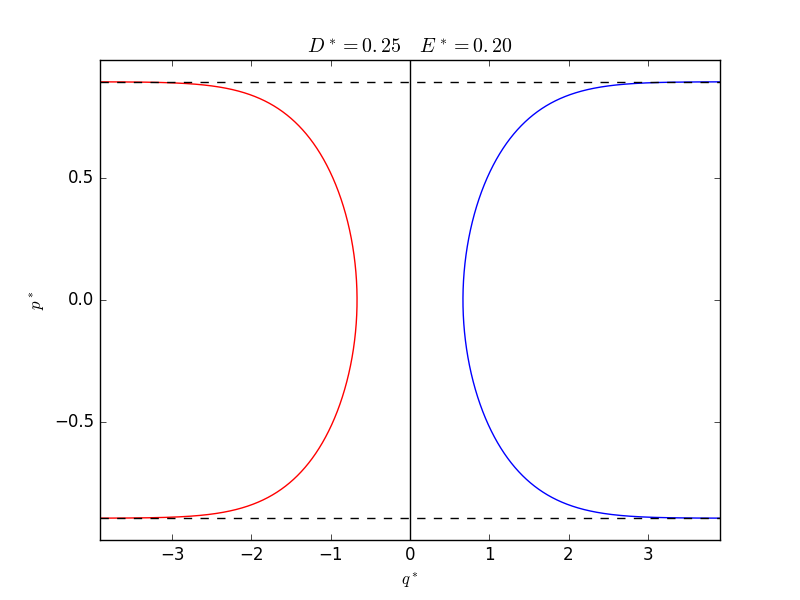
\includegraphics[trim = 7mm 0mm 17mm 10mm, clip,width=0.49\textwidth]{choque1d/curvas_teo_1.png}}
	\subfigure{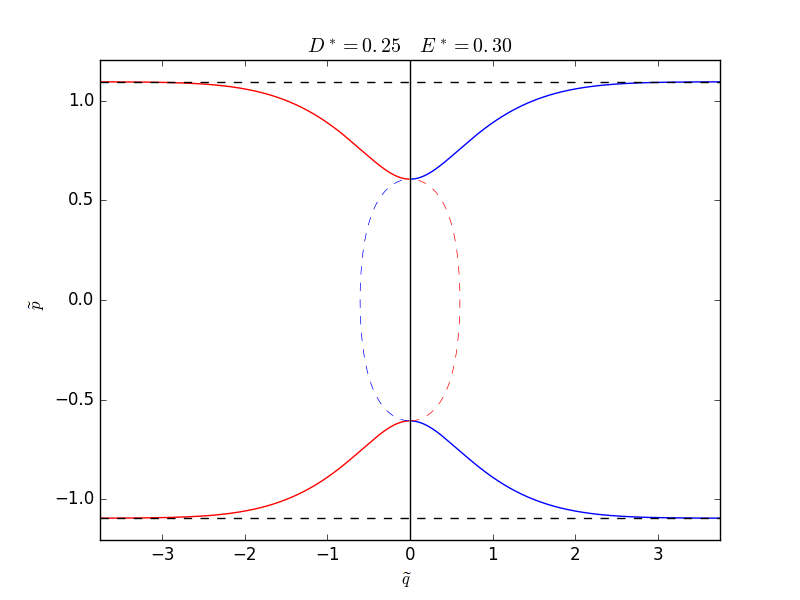
\includegraphics[trim = 7mm 0mm 17mm 10mm, clip,width=0.49\textwidth]{choque1d/curvas_teo_2.png}}
	\subfigure{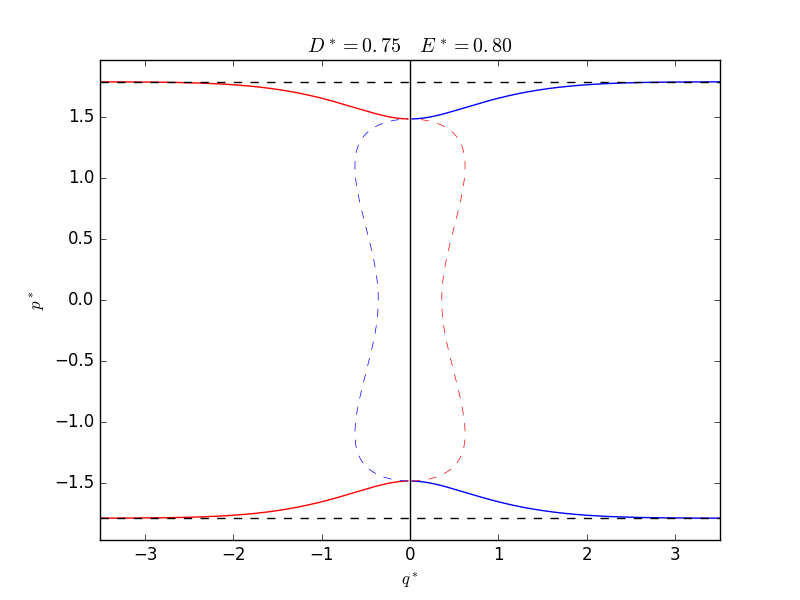
\includegraphics[trim = 7mm 0mm 17mm 10mm, clip,width=0.49\textwidth]{choque1d/curvas_teo_3.png}}
	\subfigure{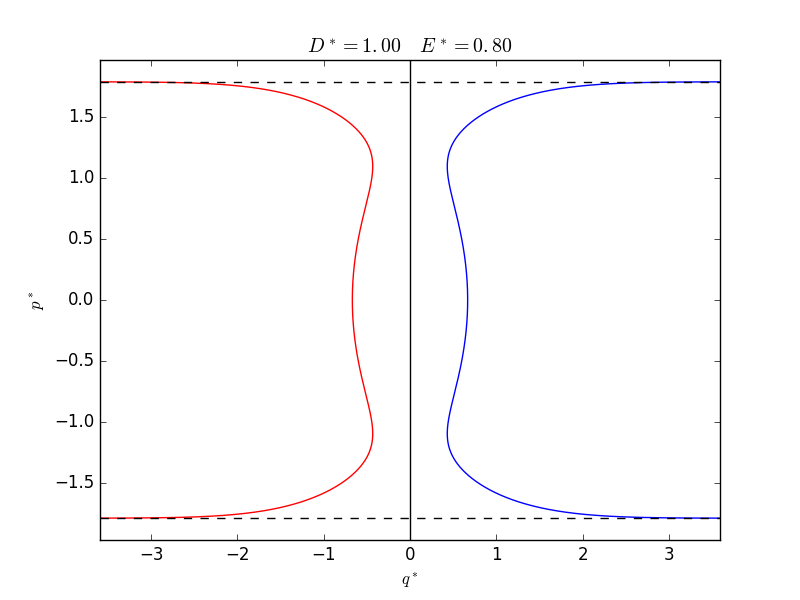
\includegraphics[trim = 7mm 0mm 17mm 10mm, clip,width=0.49\textwidth]{choque1d/curvas_teo_4.png}}
	\caption{Posibles trayectorias en el espacio de fases para los 4 casos posibles de $E^*$ y $D^*$.}
	\label{fig:curvas_teo}
\end{figure}

La existencia de región excluida para $D^*>1/2$ puede apreciarse para las curvas de doble rebote, que parecen estar circunventando el origen.
Como dijimos, a medida que $E^*\to E^*_c = (1+\log(2D^*))/2$ estas curvas acercarán sus mínimos al eje $\tilde{q}=0$ hasta transformarse en curvas de atraviese.
Es justamente para $E^*\to E^*_c $ por debajo donde los mínimos de $q\geq0$ y $q\leq0$ se conectan, encerrando la región excluida.
Por lo tanto, la curva $\tilde{q}^2(\tilde{p}; E^*=E_c^*)$ define el perímetro de esta región y podemos utilizarla para calcular el área total encerrada según
\begin{align*}
A^* = 2\int_{-\sqrt{p_\infty^2-2}}^{\sqrt{p_\infty^2-2}} \tilde{q}(p) dp \Bigg|_{p_\infty^2=4E^*_c}
= 4\int_{0}^{\sqrt{p_\infty^2-2}} \sqrt{-p^2 - 2\log\left( \frac{p_\infty^2-p^2}{2} + \log(2D^*) \right)} dp \Bigg|_{p_\infty^2=4E^*_c}
\end{align*}

Mediante el cambio de variables 
\[x = (p_\infty^2-p^2)/2\]
\[dx = -p dp \Rightarrow dp = -dx/\sqrt{p_\infty^2-2x}\] 
y usando que $p_\infty^2 = 4E^*_c$ y $\log(2D^*) = 2E_c^* - 1$ tenemos finalmente
\begin{equation}{\label{eq:area_int_ex}}
A^* = 4\int_{1}^{2E_c^*} \frac{\sqrt{-4E_c^* + 2x - 2\log(x) + 4E_c^* - 2}}{\sqrt{4E_c^* - 2x}} dx
= 4\int_{1}^{2E_c^*} \frac{\sqrt{x -1 - \log(x)}}{\sqrt{2E_c^* - x}} dx
\end{equation}
donde debemos recordar que $A^*$ es el área reducida, siendo el área total $A = q_op_oA^*$.

\begin{figure}[H]
	\centering		%trim={<left> <lower> <right> <upper>}
	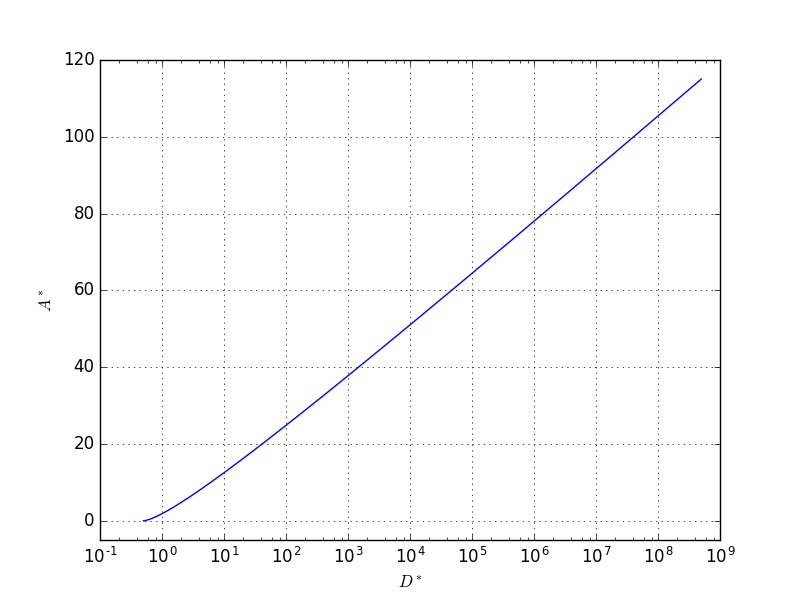
\includegraphics[trim = 10mm 2mm 15mm 12mm, clip, width=0.7\textwidth]{choque1d/AvsD_solo_teo.png}
	\caption{Área de la región excluida en función de $D^*$ obtenida de integrar numéricamente \eqref{eq:area_int_ex}. Para valores altos parece haber una relación lineal entre $A^*$ y $\log D^*$.}
	\label{fig:AvsD_teo}
\end{figure}

Sin embargo, la integral de \eqref{eq:area_int_ex} no puede expresarse como una combinación de funciones conocidas, lo cual nos impide por completo obtener una forma funcional clara.
Aún así, podemos realizar una integración numérica de $A^*$ vía regla de trapecios.
Debemos tener especial cuidado en el extremo superior, donde el integrando diverge.
El resultado de esta integración numérica en un amplio rango de $D^*$ puede apreciarse en la \textbf{Figura \ref{fig:AvsD_teo}}, donde vemos que rápidamente se cumple $A^* \approx \alpha \log(D^*) + \beta$.

Recordando las propiedades \eqref{eq:props_area_red} que esperábamos de $A^*$, es inmediato de la \textbf{Figura \ref{fig:AvsD_teo}} que $A^*$ es creciente en $D^*$.
La segunda propiedad, sin embargo, no resulta tan evidente.
En la \textbf{Figura \ref{fig:AvsD_teo_cota}} podemos apreciar el gráfico de $A^*(D^*)/\sqrt{D^*}$, donde vemos que la función se vuelve decreciente para $D^*\geq D^*_{max}\approx6.082$.
Por lo tanto, tenemos que $A$ es creciente en $p_o$ si y solo si $D^*\geq 6.082$, lo cual nos da otro criterio para elegir parte de estos parámetros. 
\begin{figure}[H]
	\centering
	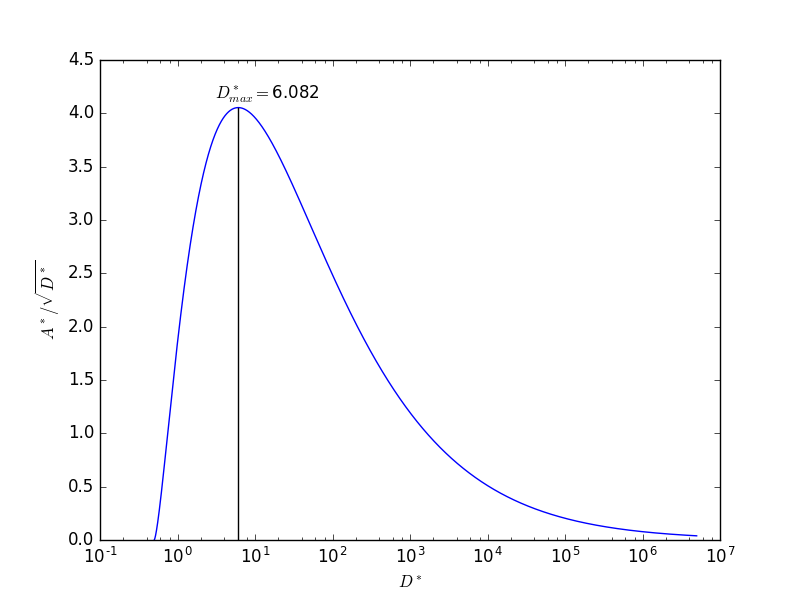
\includegraphics[trim = 9mm 2mm 15mm 12mm, clip, width=0.7\textwidth]{choque1d/Crecimiento_po.png}
	\caption{Curva de $A^*(D^*)/\sqrt{D^*}$ para confirmar la validez de la cota derecha de \eqref{eq:props_area_red}.
	Podemos ver que la función es decreciente para $D^*\geq D_{max}^* =6.082$, donde $A$ resulta entonces creciente con $p_o$.}
	\label{fig:AvsD_teo_cota}
\end{figure}

Es importante aclarar, de todos modos, que la desigualdad derecha de \eqref{eq:props_area_red}
\[ \frac{d}{dD^*} \left(\frac{A^*(D^*)}{\sqrt{D^*}}\right) \leq 0 \]
era una propiedad \textit{deseable}, pero no realmente necesaria.
Que no se cumpla implica que un aumento en $p_o$ puede generar una reducción en el área de la región excluida, pero esto no resulta particularmente problemático.
La propiedad más relevante del potencial de Pauli es la existencia de un área excluida y la capacidad de poder adaptar $D^*$ para que este área sea la buscada, lo cual ciertamente se cumple.
Si un aumento en $p_o$ genera una reducción del área excluida, es posible aumentar $D$ para corregir esto.

Más adelante retomaremos este análisis del espacio de fases desde un punto de vista computacional, simulando el choque y confirmando nuestros resultados con esta sección.




\subsection{Estudio numérico del espacio de fases}{\label{sec:num_choque_1d}}

Como dijimos, las curvas $q(p)$ del diagrama de fases mantienen el Hamiltoniano $H(q,p)$ constante.
A la hora de simular, un método que conserve la energía del sistema arrojará estas curvas $q(p)$ inmediatamente.
Una simulación de dinámica molecular evolucionando el sistema con las ecuaciones de Hamilton con un integrador simpléctico nos asegura esto, por lo que resulta más natural
que otros métodos donde la energía fluctúa (como Metropolis-Montecarlo).


\subsubsection{Implementación de integradores}{\label{sec:imp_integs}}

Según lo que discutimos en la sección \ref{sec:int_simpl}, dado que el Hamiltoniano \eqref{eq:hamiltoniano_1D} es no separable, no disponemos de integradores simplécticos y explícitos.
Con el objetivo de comparar, decidimos implementar 2 integradores no simplécticos pero explícitos y un integrador simpléctico pero no explícito.

Además, para simplificar la notación definimos \[y = \binom{p}{q} \qquad J = \begin{pmatrix}
0 & \mathbb{I} \\
-\mathbb{I} & 0
\end{pmatrix}
\]

Los integradores implementados son Euler, un Runge-Kutta de orden 2 (RK2) y MidPoint Rule (MPR).
Los esquemas pueden apreciarse junto con su información relevante en la \textbf{Tabla \ref{tab:integradores}}.
La simplecticidad de MPR fue probada en \ref{sec:int_simpl} mientras que la no simplecticidad de Euler y RK2 se encuentra en el \textbf{Apéndice \ref{sec:no_simp}}.

\begin{table}[h]
	\centering
	\begin{tabular}{|c|c|c|c|c|}
		\hline
		\textbf{Integrador} & \textbf{Esquema} & \textbf{Orden} & \textbf{¿Explícito?} & \textbf{¿Simpléctico?} \\ \hline
		Euler & $ y_{n+1} = y_n + hJ^{-1}\nabla H(y_n)$ & $1$ & Si & No \\ \hline
		Runge-Kutta 2 & $y_{n+1} = y_n + hJ^{-1}\nabla H\left(y_n+\frac{h}{2}\nabla H(y_n) \right)$ & $2$ & Si & No \\ \hline
		Midpoint Rule & $y_{n+1} = y_n +  hJ^{-1}\nabla H\left(\frac{y_n+y_{n+1}}{2} \right)$ & $2$ & No & Si \\ \hline
	\end{tabular}
	\caption{Información sobre los integradores utilizados}
	\label{tab:integradores}
\end{table}

Dado que no es explícito, para el integrador MPR implementamos además un método de punto fijo para poder resolver cada paso.
Sumando $y_n$ a cada lado del esquema MPR y dividiendo por 2, podemos redefinir $Z = \frac{y_n+y_{n+1}}{2}$ tal que
\[ Z = y_n + \frac{h}{2}J\nabla H(Z) \equiv F(Z) \]
y resolver esta ecuación de punto fijo con parámetro conocido $y_n$ en \textit{cada iteración} evaluando múltiples veces $F(Z)$.
En principio, puede probarse que $|DF(Z)|<1$ (punto fijo converge) para $h$ suficientemente chico dado que el Hessiano del potencial de Pauli está acotado (es gaussiano).
Sin embargo, la cota para $h$ dependerá de los parámetros $p_o$, $q_o$ y $D$ e incluso podría depender del número de partículas $N$ del sistema.
Por lo tanto, en principio nos conformaremos con saber que tal $h$ existe e intentar encontrarlo según la situación.

En lo que sigue, siempre resolvimos el problema de punto fijo $Z = F(Z)$ utilizando $k=5$ iteraciones, al notar que valores más altos de $k$ no mejoraban apreciablemente la convergencia.
Cabe aclarar, sin embargo, que sistemas con más partículas pueden \textit{a priori} exigir valores mayores de $k$.

\subsubsection{Conservación de la energía}

A modo de comparación, corrimos una simulaciones del choque de 2 partículas en 1D, muestreando el Hamiltoniano (de ahora en más, la energía) a lo largo del recorrido.
Consistentemente con lo que vimos en la sección \ref{sec:teo_fases}, durante el choque de 2 partículas pueden darse 2 situaciones: rebote o atraviese, dependiendo del valor inicial del Hamiltoniano $E$ y el valor de $D$.

Dado que nos interesa trabajar con potenciales de Pauli con región excluida, configuramos el potencial de Pauli con $D = 10000$ y aprovechamos la adimensionalización para tomar $qo = 1 = po = m$ tal que 
$D^*=D>1/2$.
En este caso particular, analizaremos un atraviese.
El sistema comienza con una de las partículas en el origen con impulso nulo (en la posición $(0, 0)$ del espacio de fases) y otra a distancia $6$ e impulso $-4$ (en el $(6, -4)$).

\begin{figure}[H]
	\centering
	\subfigure[Euler]{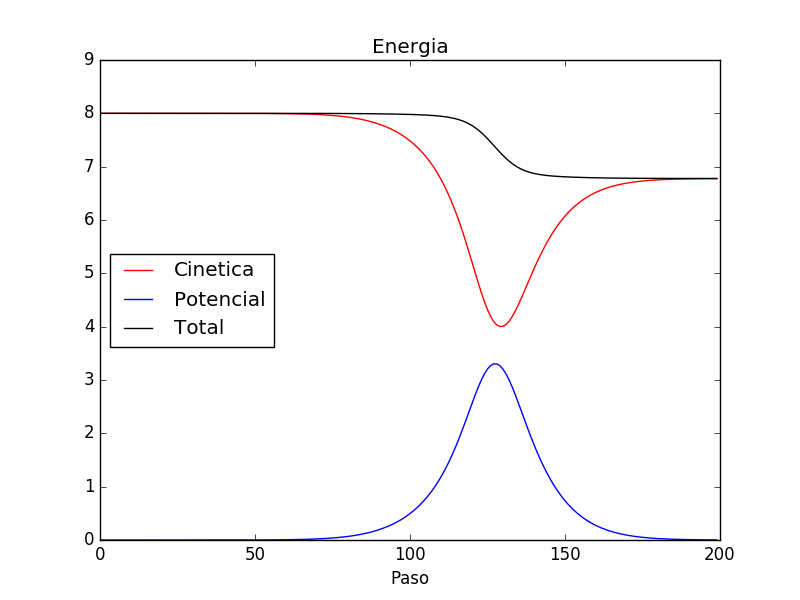
\includegraphics[trim = 20mm 0mm 15mm 10mm, clip, width=0.325\columnwidth]{choque1d/energia_euler_0,01.png}}
	\subfigure[Runge-Kutta 2]{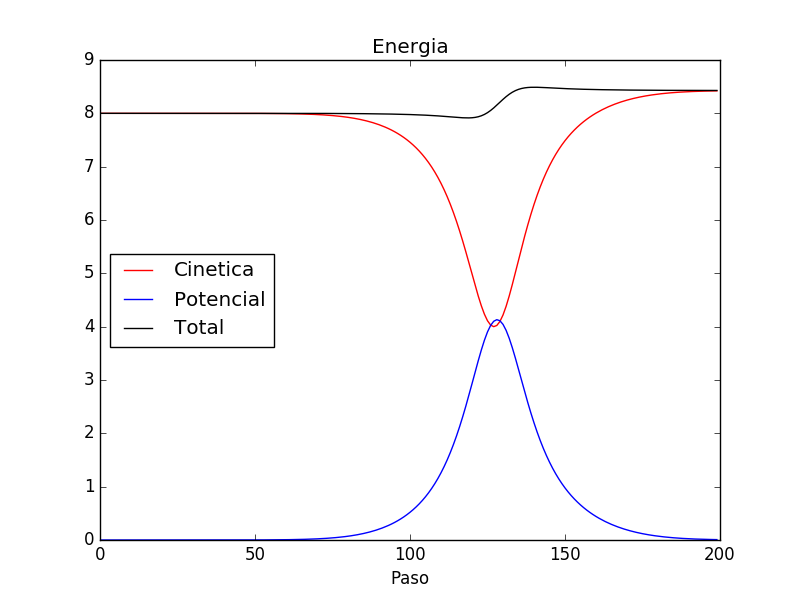
\includegraphics[trim = 20mm 0mm 15mm 10mm, clip, width=0.325\columnwidth]{choque1d/energia_rk2_0,01.png}}
	\subfigure[Midpoint Rule]{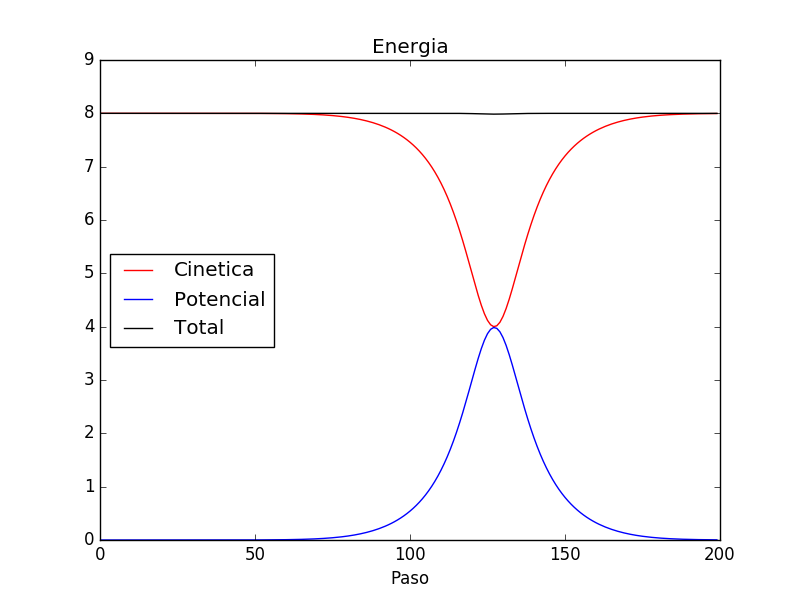
\includegraphics[trim = 20mm 0mm 15mm 10mm, clip, width=0.325\columnwidth]{choque1d/energia_mpr_0,01.png}}
	\caption{Energía durante un choque para un potencial de Pauli con $D = 10000$ y $qo = 1 = po = m$. La trayectoria comenzó en el $(q, p) = (6, -4)$, integrada con paso temporal $h=0.01$}
	\label{fig:energ_choq}
\end{figure}

A modo de ejemplo y para visualizar el problema, en la \textbf{Figura \ref{fig:energ_choq}} puede apreciarse la energía durante un choque para paso temporal $h=0.01$.
Es interesante notar que RK2 tiende a aumentar $E$ mientras que Euler tiende a disminuirla; está clara la mayor efectividad de MPR.

Realizamos estos choques para distintos valores de $h$ (y las mismas condiciones iniciales) y analizamos la fluctuación relativa de energía (siempre positiva para este hamiltoniano).
Los resultados pueden apreciarse en la \textbf{Figura \ref{fig:flucvsh}}, donde se confirma la clara superioridad de MPR a la hora de conservar la energía.
Esto último resulta a priori esperable dado que MPR es un integrador simpléctico; no obstante, al ser resuelta la ecuación con un método de punto fijo, esto pudo haber dejado de ser cierto.
Aún así, vemos un cierto rebote para $h\leq10^{-3}$, mostrando que el error relativo comienza a empeorar para $h$ demasiado pequeño.
Esto es llamativo, pero probablemente se deba a complicaciones a la hora de resolver la ecuación implícita mediante punto fijo; es posible que deba tomarse un número $k$ de iteraciones mayor
para valores tan pequeños de $h$.

\begin{figure}[H]
	\centering
	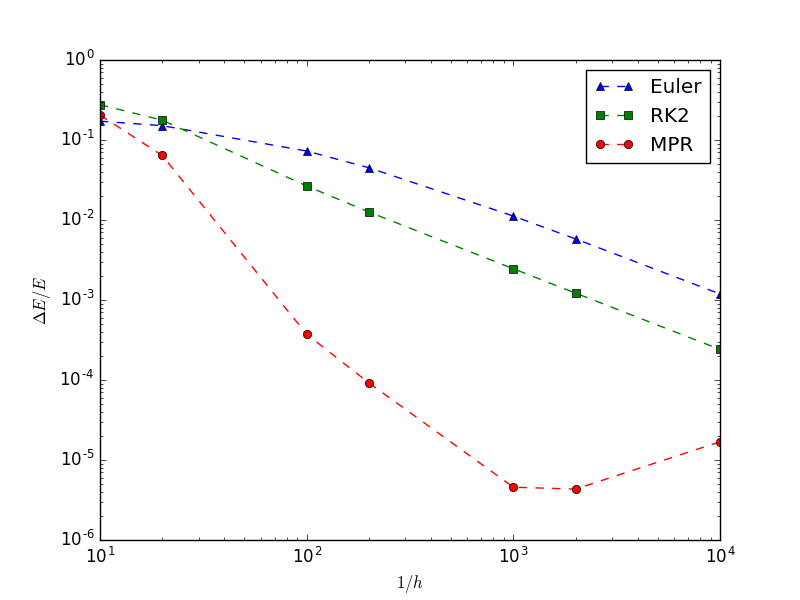
\includegraphics[trim = 0mm 0mm 15mm 10mm, clip, width=0.6\columnwidth]{choque1d/fluct_vs_h.png}
	\caption{Fluctuaciones de energía en función de paso temporal para distintos integradores.
	El integrador MPR se muestra superior en todo el rango, pero vuelve a crecer para $h\leq10^{-3}$, probablemente debido a errores al resolver la ecuación implícita.}
	\label{fig:flucvsh}
\end{figure}

\subsubsection{Primeros diagramas de fases}

Como dijimos, al ser un sistema unidimensional $(q,p)$, el diagrama de fases queda definido univocamente por $H(q,p)\equiv E = \text{cte}$.
Por lo tanto, la conservación de la energía por parte de los integradores resulta suficiente para obtener estas curvas $q(p)$ y así construir el diagrama.
Con este objetivo, configuramos el sistema inicialmente con una partícula en el $(0,0)$ y la otra en un valor $(q_i, p_i)$.
Luego, evolucionamos el sistema muestreando los valores de $q = q_1 - q_2$, $p = p_1 - p_2$.

\begin{figure}[H]
	\centering	%trim={<left> <lower> <right> <upper>}
	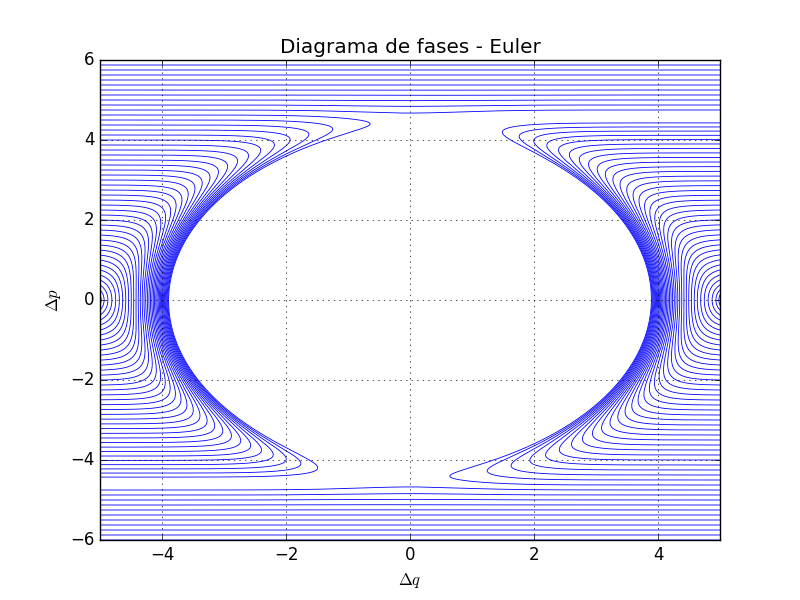
\includegraphics[trim = 11mm 0mm 20mm 5mm, clip, width=0.495\textwidth]{choque1d/fases_Euler.png}
	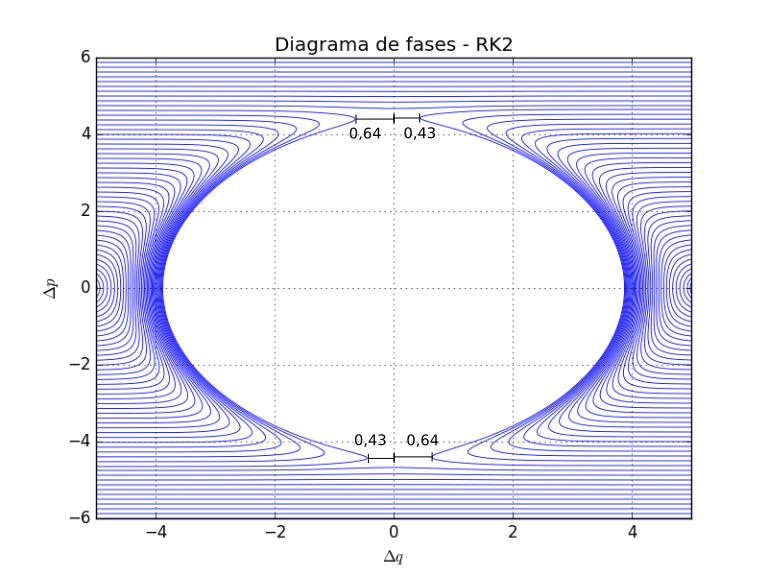
\includegraphics[trim = 11mm 0mm 20mm 5mm, clip, width=0.495\textwidth]{choque1d/fases_RK2_marcado.png}
	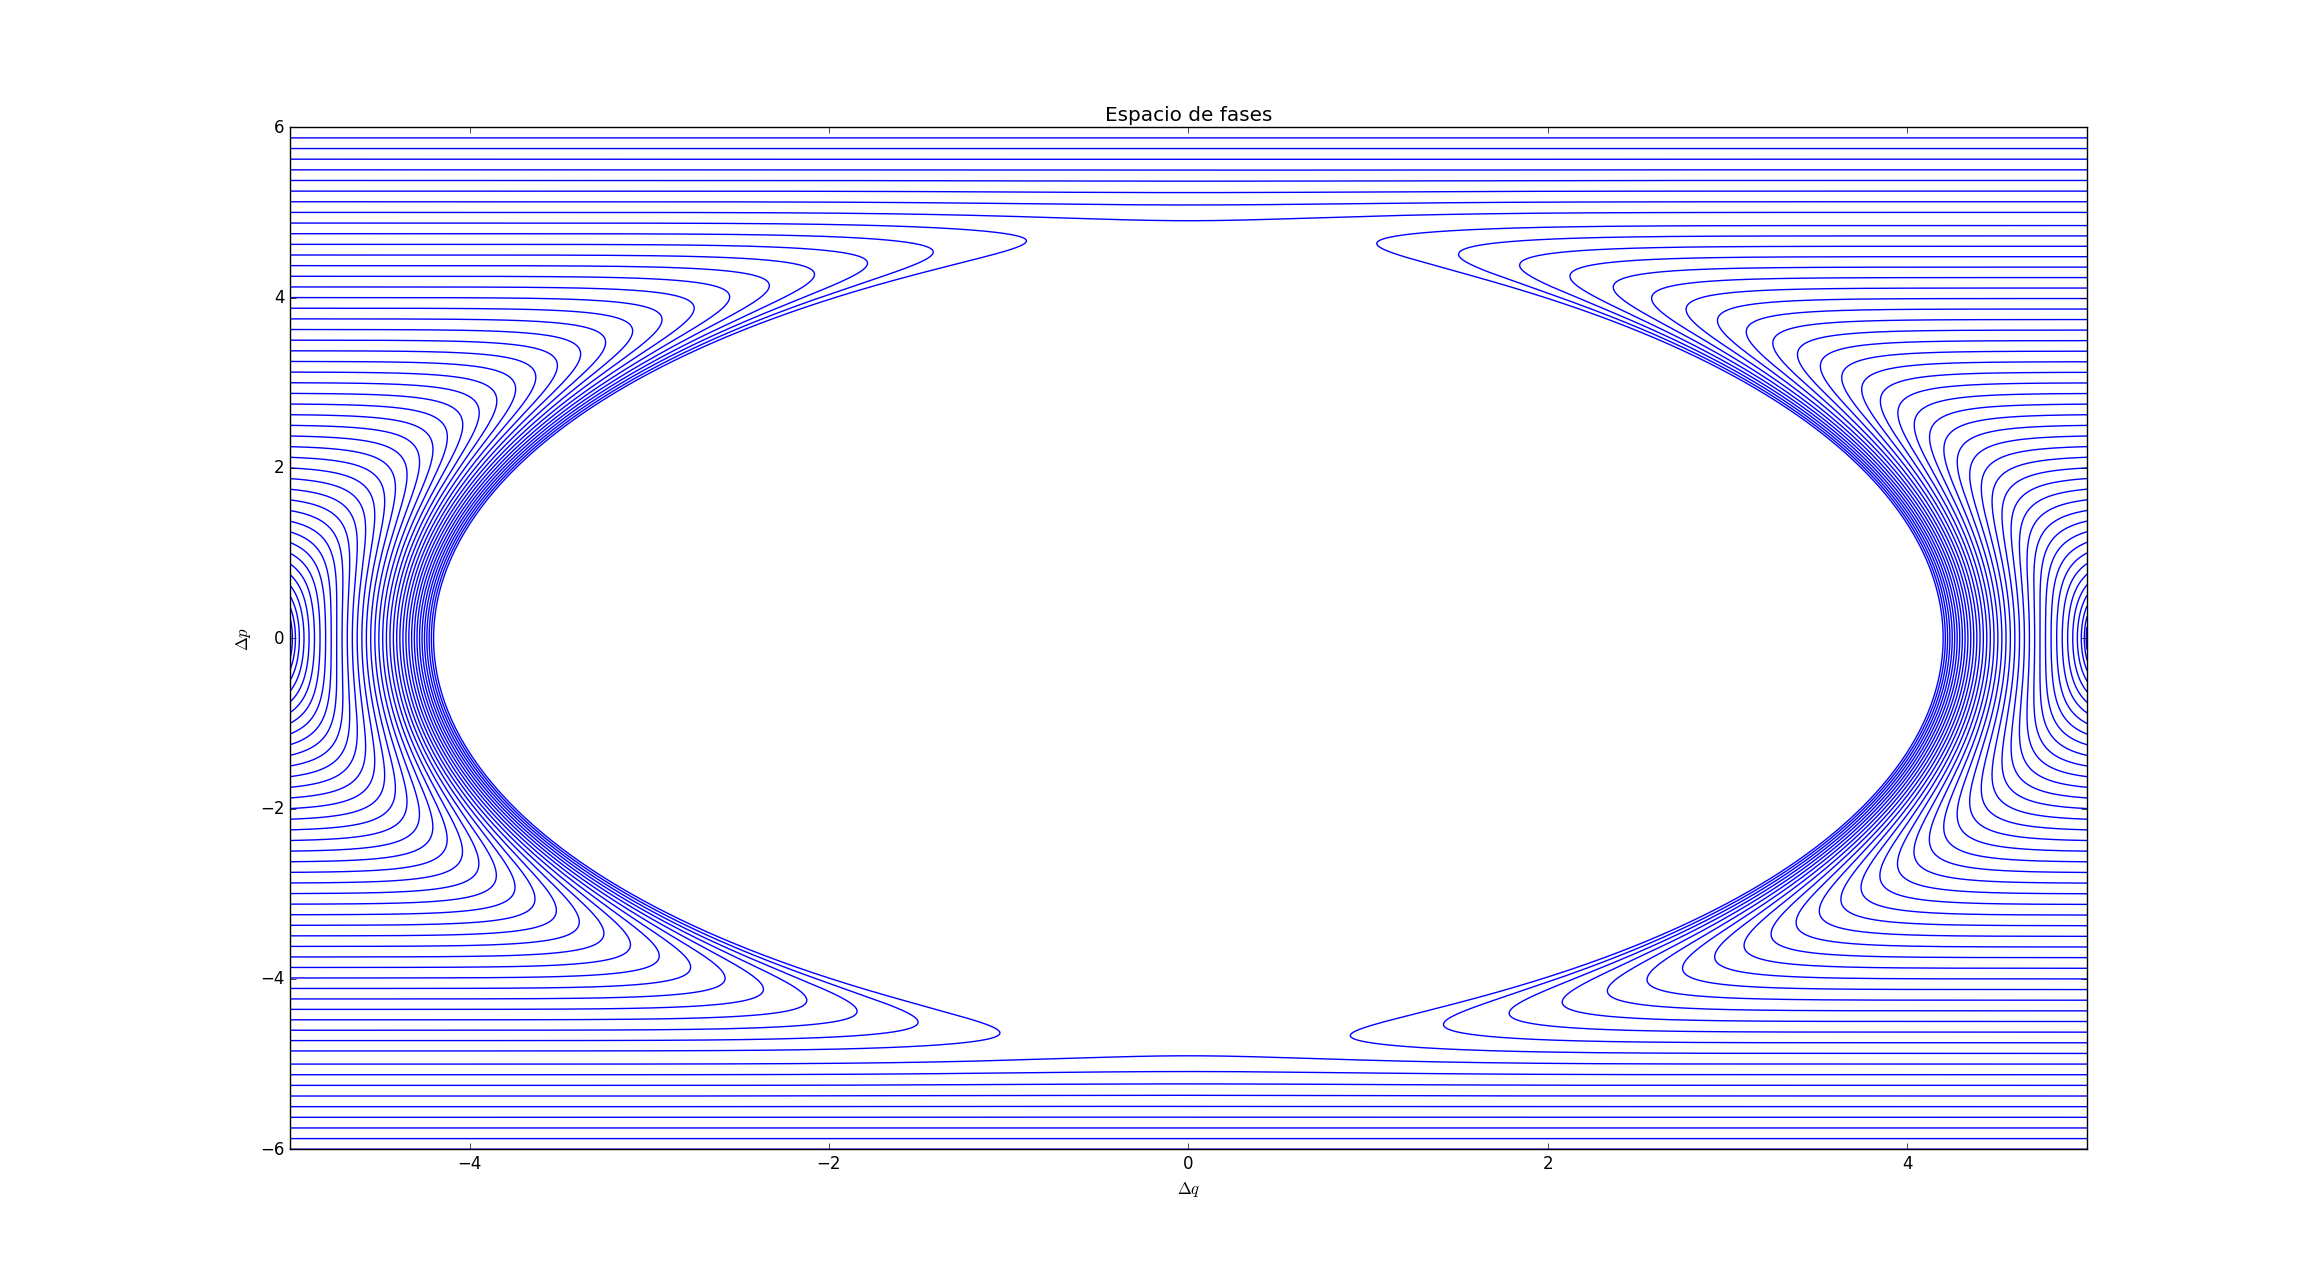
\includegraphics[trim = 11mm 0mm 20mm 5mm, clip, width=0.6\textwidth]{choque1d/fases.png}
	\caption{Diagrama de fases para $D=10000$, $m=1=p_o=q_o$ y $h=10^{-3}$. Además de la zona inaccesible, se evidencian las curvas de rebote y atraviese según lo previsto en \ref{sec:teo_fases}.
		Sin embargo, los métodos de Euler y RK2 no preservan la simetría ante reflexiones en $q$ y $p$.
		Para RK2 están marcadas las distancias en $q$ de la curva de rebote más cercana}
	\label{fig:ej_diag_fases}
\end{figure}

Tomamos entonces un rango de condiciones iniciales $(q_i,p_i)=(5,p)$ con $p\in [-6,0]$ y analizamos las curvas $q(p)$ resultantes, sabiendo que el cambio de $p$ se traduce en un cambio de $E$.
Mantuvimos $q_i=5$ fijo dado que así emulábamos una colisión desde el infinito, dado que podemos considerar que $V_P(5,p)\leq 4\times10^{-6}D \ll D$ es nulo.
Utilizamos los mismos parámetros para el potencial de Pauli ($D=10000$, $m=1=p_o=q_o$) por consistencia.
Hicimos esto una vez para cada integrador para así poder comparar la calidad de los diagramas de fases, siempre con paso $h=10^{-3}$.
En la \textbf{Figura \ref{fig:ej_diag_fases}} podemos ver estas curvas superpuestas en nuestros primeros diagramas de fases.

El caso de Euler es notoriamente malo, donde se aprecian franjas desocupadas que no deberían existir.
Estas franjas indican que el integrador no pudo preservar apropiadamente la energía, dado que el $p^2$ posterior al choque es menor al inicial, lo cual concuerda con lo visto en la \textbf{Figura \ref{fig:energ_choq}}.
El caso de RK2 es menos apreciable, pero ciertamente hay una asimetría entre $q$ y $-q$ dado que los puntos de mayor cercanía de las curvas de rebote no están espejados respecto de $q=0$ como marcamos en la \textbf{Figura \ref{fig:ej_diag_fases}}.
Ciertamente, el integrador MPR genera un diagrama de fases que respeta mejor las simetrías de reflexión en $q$ y $p$, consistente con su capacidad para conservar la energía que vimos en \ref{fig:energ_choq}.

Independientemente de esta simetría, es fundamental notar que el diagrama se compone de dos tipos de curva: rebotes y atravieses.
En particular, los rebotes tienen dos puntos de máxima cercanía, en perfecta concordancia con lo analizado en \ref{sec:teo_fases} dado que tenemos $D^*=10^4>1/2$.
Incluso puede verse que la transición de rebote a atraviese (para MPR) ocurre para $4.625\leq p_i\leq4.75$, consistente con
\[ E_c = \frac{p_i^2}{4} = \frac{1}{2}\left( 1 + \log(2D) \right) \approx 5.45 \Longrightarrow p_i \approx 4.67 \]

Veremos en la sección \ref{sec:area_ex_comp} que no solo se verifica esto sino también el área total excluida, cuyo cómputo tiene sus propias complicaciones.


\subsubsection{Conservación del volumen de fases}

Como discutimos en la sección \ref{sec:trans_simp}, la simplecticidad de las ecuaciones de Hamilton asegura no solo la conservación de la energía, sino la conservación del volumen orientado \eqref{eq:area_orien_simp}.
Esto conlleva, en otras cosas, al Teorema de Liouville y la conservación del volumen de fases.
La evolución de una dada región de condiciones iniciales en el espacio de fases preserva su volumen total.

Por lo tanto, otro criterio para calificar la efectividad de los integradores es la conservación del volumen de fases a lo largo de la evolución.
Para esto, realizamos una simulación tomando un conjunto de valores iniciales $(q_i, p_i)$ y evolucionándolos paralelamente en el tiempo.
Asumimos que cada uno de los puntos era el centro de una elipse rígida de ejes definidos, de forma que la región total asociada al conjunto era la unión de estas elípses.
Así, calculamos para cada tiempo el volumen de esta región total para poder analizar su evolución en el tiempo.

Hicimos esto para curvas de rebote (doble) con 81 condiciones iniciales en un cuadrado de $0.04\times0.04$ alrededor del $(6, -4)$ y los mismos parámetros de antes para Pauli.
Tomamos estas elipses suficientemente grandes como para cubrir completamente este cuadrado inicial, por lo que hubo considerable superposición de volúmenes.
Los resultados pueden apreciarse en la \textbf{Figura \ref{fig:vol_fas}}.

\begin{figure}[h]
	\centering
	\subfigure[h = 0.01]{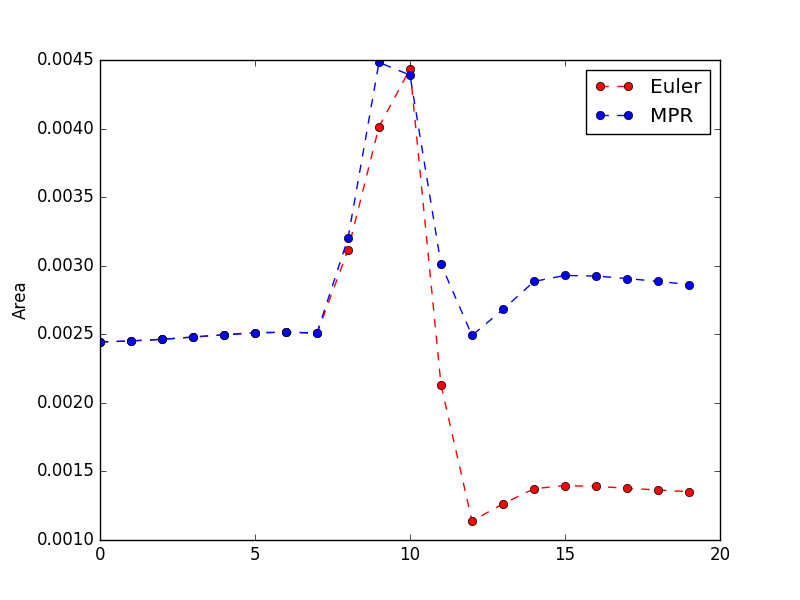
\includegraphics[trim = 0mm 0mm 15mm 10mm, clip, width=0.32\columnwidth]{choque1d/vol_fas_0,01.png}}
	\subfigure[h = 0.005]{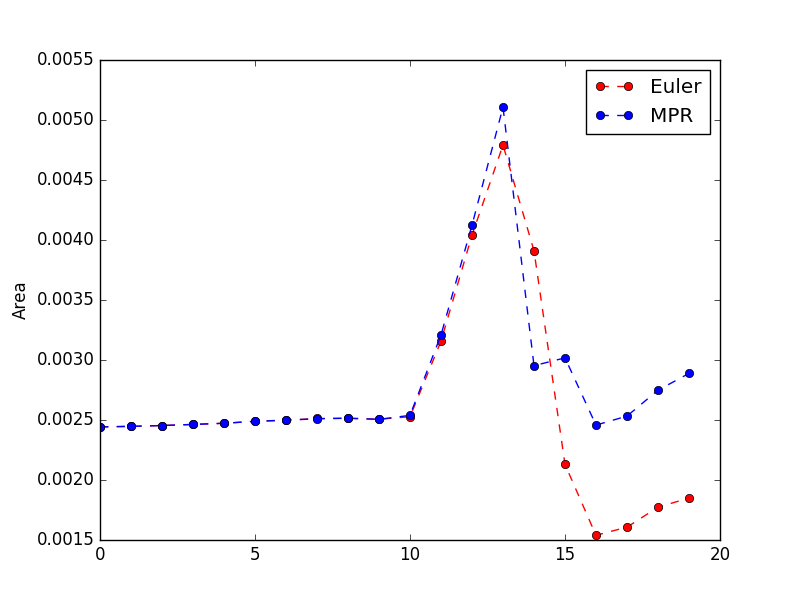
\includegraphics[trim = 0mm 0mm 15mm 10mm, clip, width=0.32\columnwidth]{choque1d/vol_fas_0,005.png}}
	\subfigure[h = 0.001]{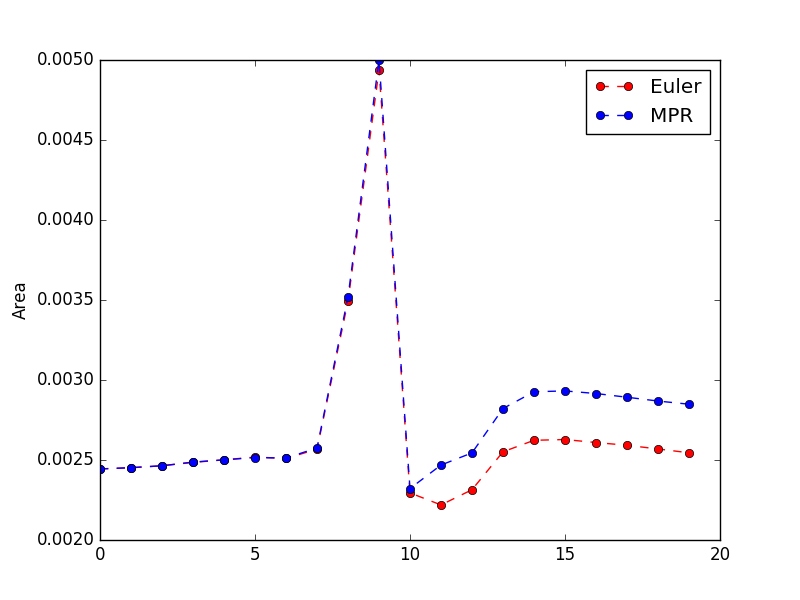
\includegraphics[trim = 0mm 0mm 15mm 10mm, clip, width=0.32\columnwidth]{choque1d/vol_fas_0,001.png}}
	\caption{Volumen de un conjunto de puntos a lo largo de una curva de rebote. El pico corresponde al momento de máxima interacción.}
	\label{fig:vol_fas}
\end{figure}

Lo primero que podemos notar es la existencia de un pico, que corresponde los instantes de mayor interacción entre las partículas.
Sin embargo, es importante notar que luego de ello los volúmenes recuperan su valor inicial.
Esto es un buen indicio y ocurre para $h=10^{-3}$ para ambos integradores, pero solo para el MPR en los otros 2 casos.
En un tercer caso con $h=0.1$ (grande) que omitimos, ninguno de los 2 métodos cumplía esto.

Para comprender este pico, nos basta analizar la \textbf{Figura \ref{fig:ej_diag_fases}} y notar que entre rebotes se da la mayor interacción.
En esta región, las curvas de nivel se comprimen, aumentando considerablemente su densidad.
Es por esto que nuestro conjunto de puntos (inicialmente dispuestos en un cuadrado) tiende a alinearse en una figura predominantemente unidimensional, donde resulta claro que el cálculo del área
no es apropiada y genera una sobreestimación de la misma.

Sin embargo, nos resulta suficiente notar que el volumen de fases se conserva luego de cada choque, donde vemos nuevamente que el integrador MPR tiene una mayor robustez,
manteniendo las propiedades de una evolución simpléctica para valores de $h$ mayores comparado a Euler.


\subsection{Área excluida}{\label{sec:area_ex_comp}}

Con el objetivo de obtener $A^*(D^*)$ de la simulación, nuevamente tomaremos $q_o = p_o = m = 1$ de forma que $D^* = D$ y $A=A^*$.
De esta manera, solo es necesario calcular el área de la región excluida.
Para esto, sin embargo, es necesario identificar la curva $C$ de rebote que define esta región.
Para simplificar la notación, definimos la curva $C(q_i,p_i)$ como la curva de energía constante $H(q_i,p_i)$; la curva sobre la que evoluciona el sistema.
De esta manera, la curva $C(q_i,p_i)$ puede pensarse como la que describe el sistema con condiciones iniciales $(q_i,p_i)$.

Con esto en mente, corremos simulaciones que muestreen las curvas $C$ para encontrar el mayor valor de $p_i$ tal que $C(q_i, p_i)$ es un rebote.
Como antes, fijaremos $q_i=5$ pero no discriminaremos entre rebotes simples y dobles, dado que moveremos $D^*$ por encima y por debajo de $1/2$.
Realizamos esta búsqueda en forma binaria, tomando un $p_{max}$ que cumpla que $C(q_i, p_{max})$ sea un atraviese, sabiendo que $C(q_i, 0)$ \textbf{\textit{siempre}} es un rebote.
Obtenemos el $p_{max}$ tomando un valor inicial $p_{max} = -3$ y duplicándolo hasta obtener un atraviese.
Con estos 2 valores de impulso, iteramos la búsqueda binaria hasta que $|p_{max}-p_{min}|\leq tol$.
El valor de $tol$ resulta arbitrario, por lo que tomamos uno dependiente de $D^*$ según $tol \sim \sqrt{D^*}\times 10^{-4}$, pues nos resultó eficiente a lo largo del proceso.
El paso temporal fue $h=10^{-3}$ para $D\leq 1000$, $h=5\times10^{-3}$ para $5000\leq D\leq 50000$ y $h=10^{-4}$ para $D\geq 100000$.

\begin{figure}[H]
	\centering
	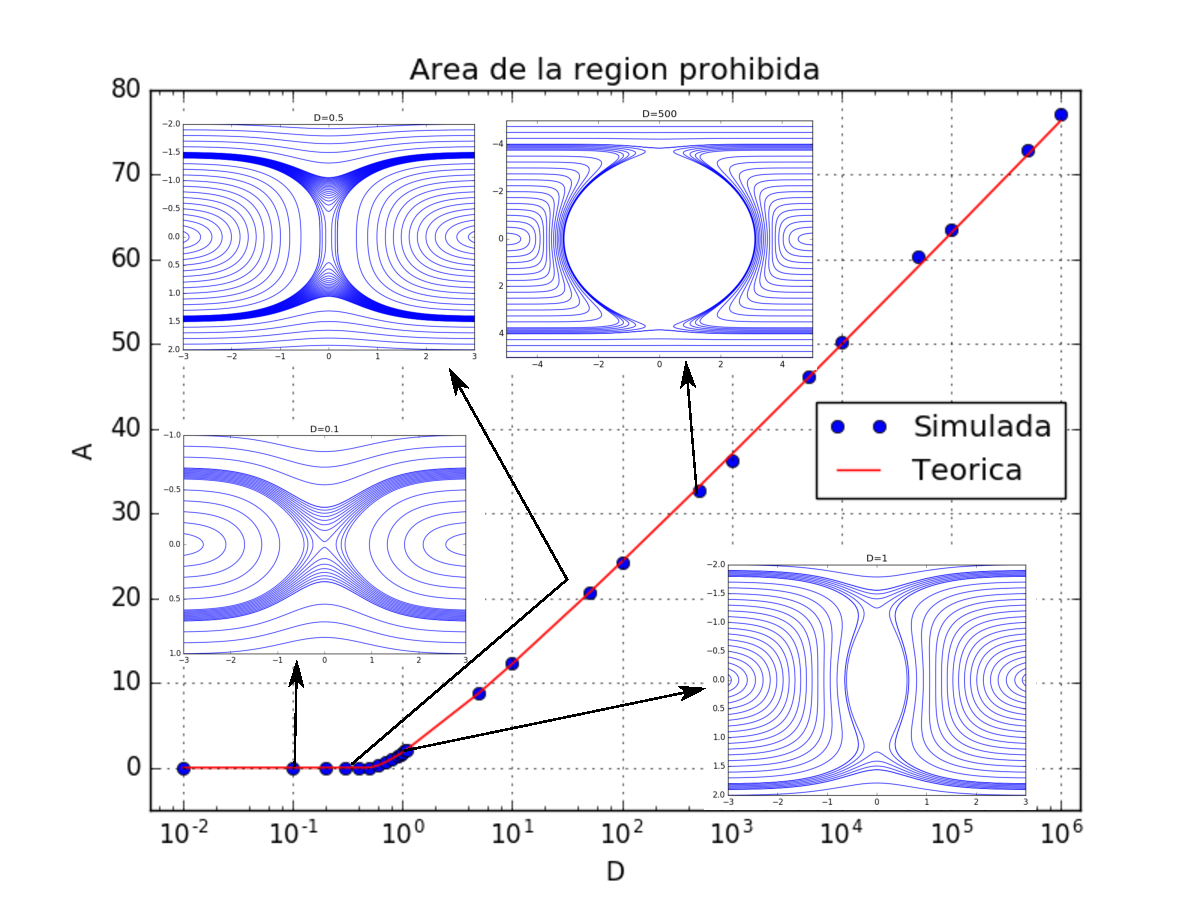
\includegraphics[trim = 0mm 0mm 15mm 10mm, clip, width=\columnwidth]{choque1d/AvsD_full_teo.pdf}
	\caption{Área prohibida en función de intensidad de potencial junto con algunos de los espacios de fase asociados.
		Tenemos $A^*=0$ para $D\leq 0.5$ y $A\sim \log{D^*}$ para $D\geq 1$ en perfecto acuerdo con la formulación teórica.}
	\label{fig:AvsD}
\end{figure}

Denominamos $p_b$ al impulso resultado de esta búsqueda, cumpliendo que tenemos un rebote para $p\leq p_b$ y un atraviese para $p>p_b$.
Teniendo la curva $C(q_i, p_b)$, la reescribimos como $q(p)$ e integramos para $p\in[-p_{min},p_{min}]$ donde $q(p_{min})=0$ utilizando una regla de trapecios para obtener el área $A^*/2$ (pues tenemos la mitad izquierda de la región excluida).
Ciertamente, estamos aprovechando las simetrías de reflexión que vimos que MPR poseía.

Los resultados pueden apreciarse en la \textbf{Figura \ref{fig:AvsD}} junto con algunos ejemplos del espacio de fases.
En la misma figura está nuevamente el gráfico del área según el cálculo teórico, que resulta concordante.
La primera observación es que $A=0$ para $D\leq 0.5$, donde las curvas de rebote son cóncavas (rebote simple, $p_{min}=0$) para $q\approx 0$ a diferencia del caso $D\geq 0.5$ donde son convexas
(para rebote doble, como en el ejemplo de la \textbf{Figura \ref{fig:ej_diag_fases}}).
De hecho, puede apreciarse que para $D=0.5$, las curvas son prácticamente verticales, marcando este cambio de convexidad.

\begin{figure}[H]
	\centering
	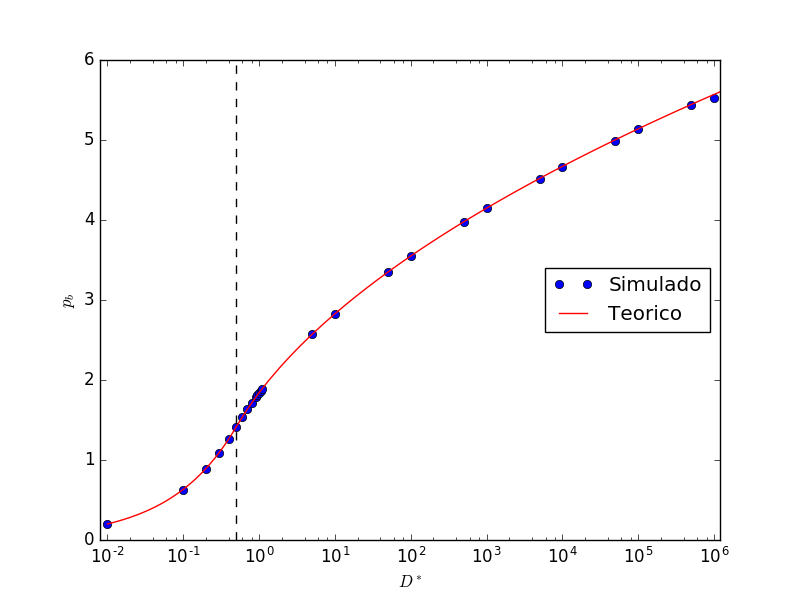
\includegraphics[trim = 0mm 0mm 15mm 10mm, clip, width=0.75\columnwidth]{choque1d/pinfvsD.png}
	\caption{Impulso crítico de transición (en módulo) rebote-atraviese en función de intensidad de potencial junto con el valor teórico, con el que coincide
	correctamente. La linea punteada marca $D^*=1/2$, donde la forma funcional de $p_b$ cambia.}
	\label{fig:pbvsD}
\end{figure}

Paralelamente, podemos graficar los valores de $p_b$ obtenidos.
En particular, es $E_c = p_b^2/4$, por lo que según vimos en \ref{sec:teo_fases} tiene forma de función partida.
\[p_b(D^*) =\left\{\begin{matrix}
2\sqrt{D^*} & D^*\leq 0,5 \\
\sqrt{2(1+\log(2D^*))} & D^*> 0,5
\end{matrix}\right.\]

La comparación del valor obtenido por la simulación con el teórico se encuentra en la \textbf{Figura \ref{fig:pbvsD}}.
Ambos coinciden dentro del (amplio) rango estudiado, lo cual termina de mostrarnos la efectividad de MPR a la hora de integrar las ecuaciones de movimiento.